%
\begin{figure}%
\centering%
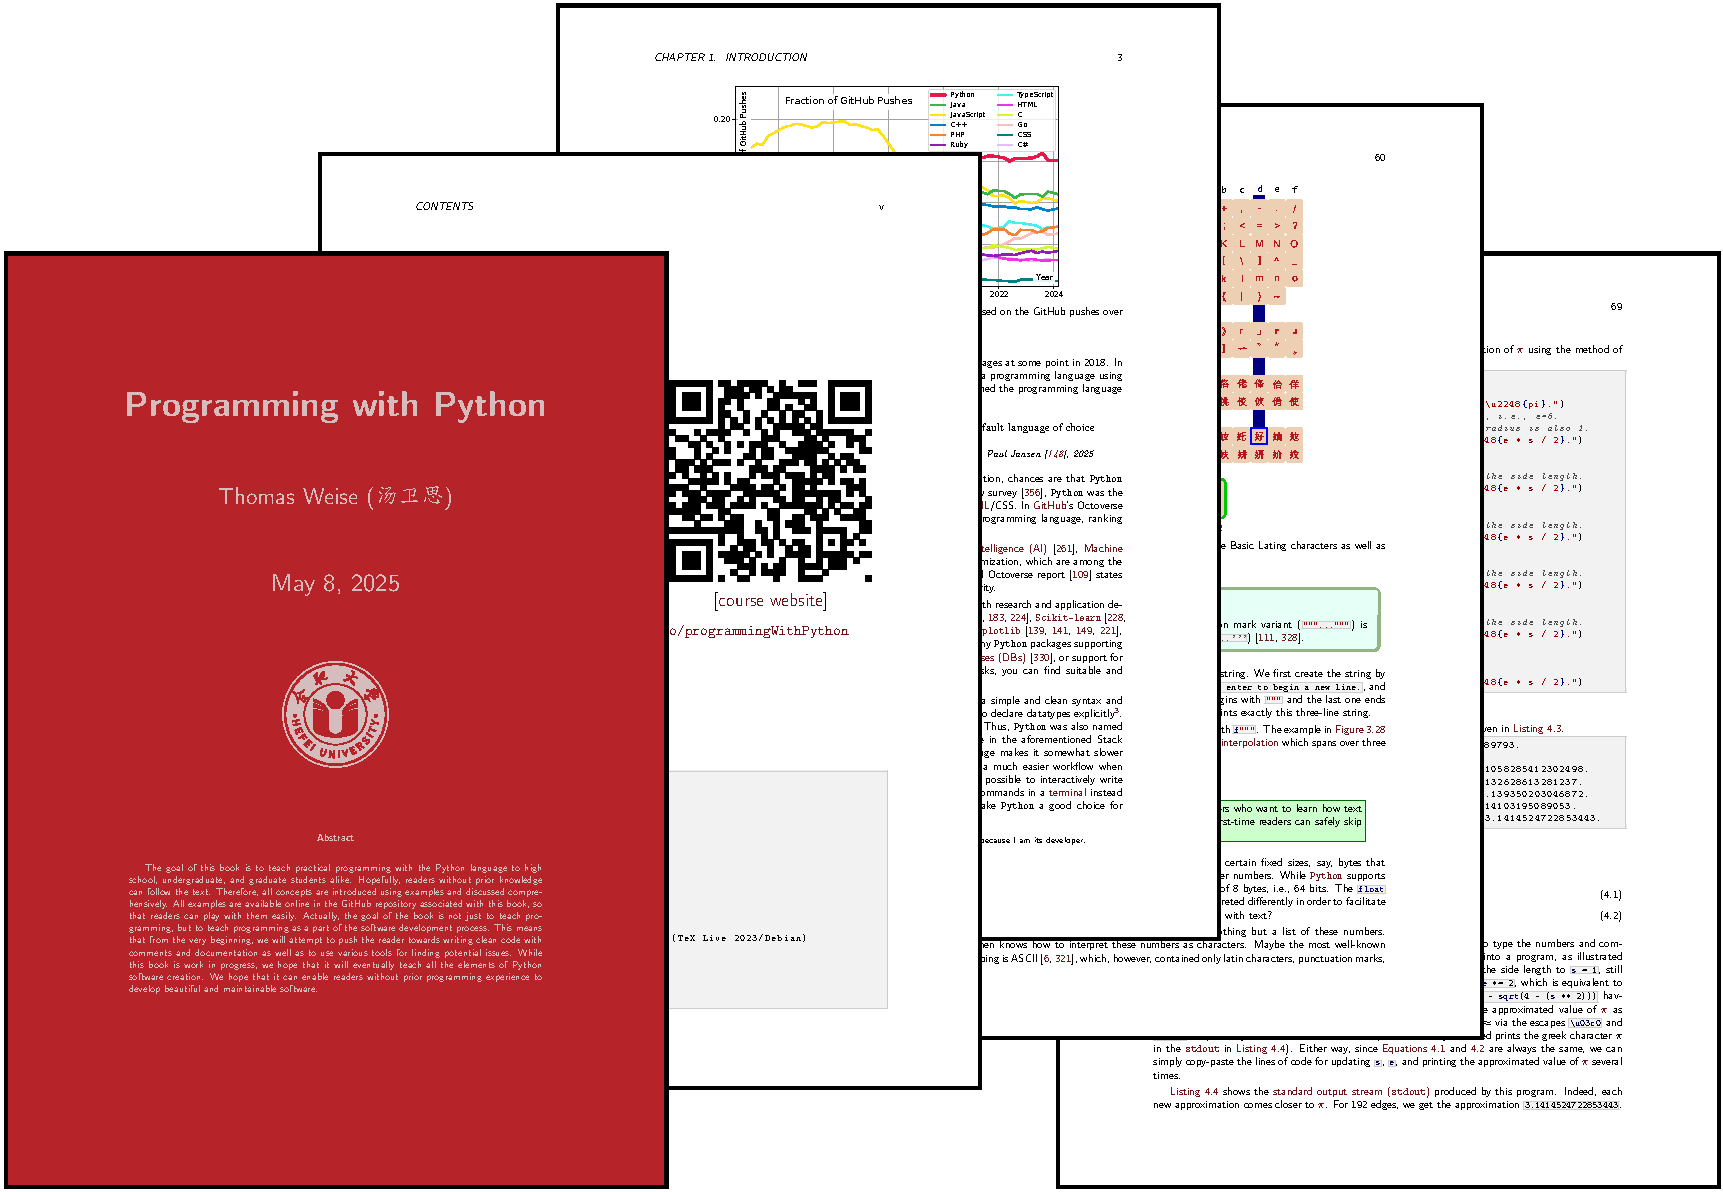
\includegraphics[width=0.6\linewidth]{\currentDir/documentDataProgrammingWithPython}%
\caption{An example of an unstructured document data in form of some pages of the book~\citetitle{programmingWithPython}~\cite{programmingWithPython}.}%
\label{fig:documentDataProgrammingWithPython}%
\end{figure}%
%
\begin{figure}%
\centering%
\tightbox{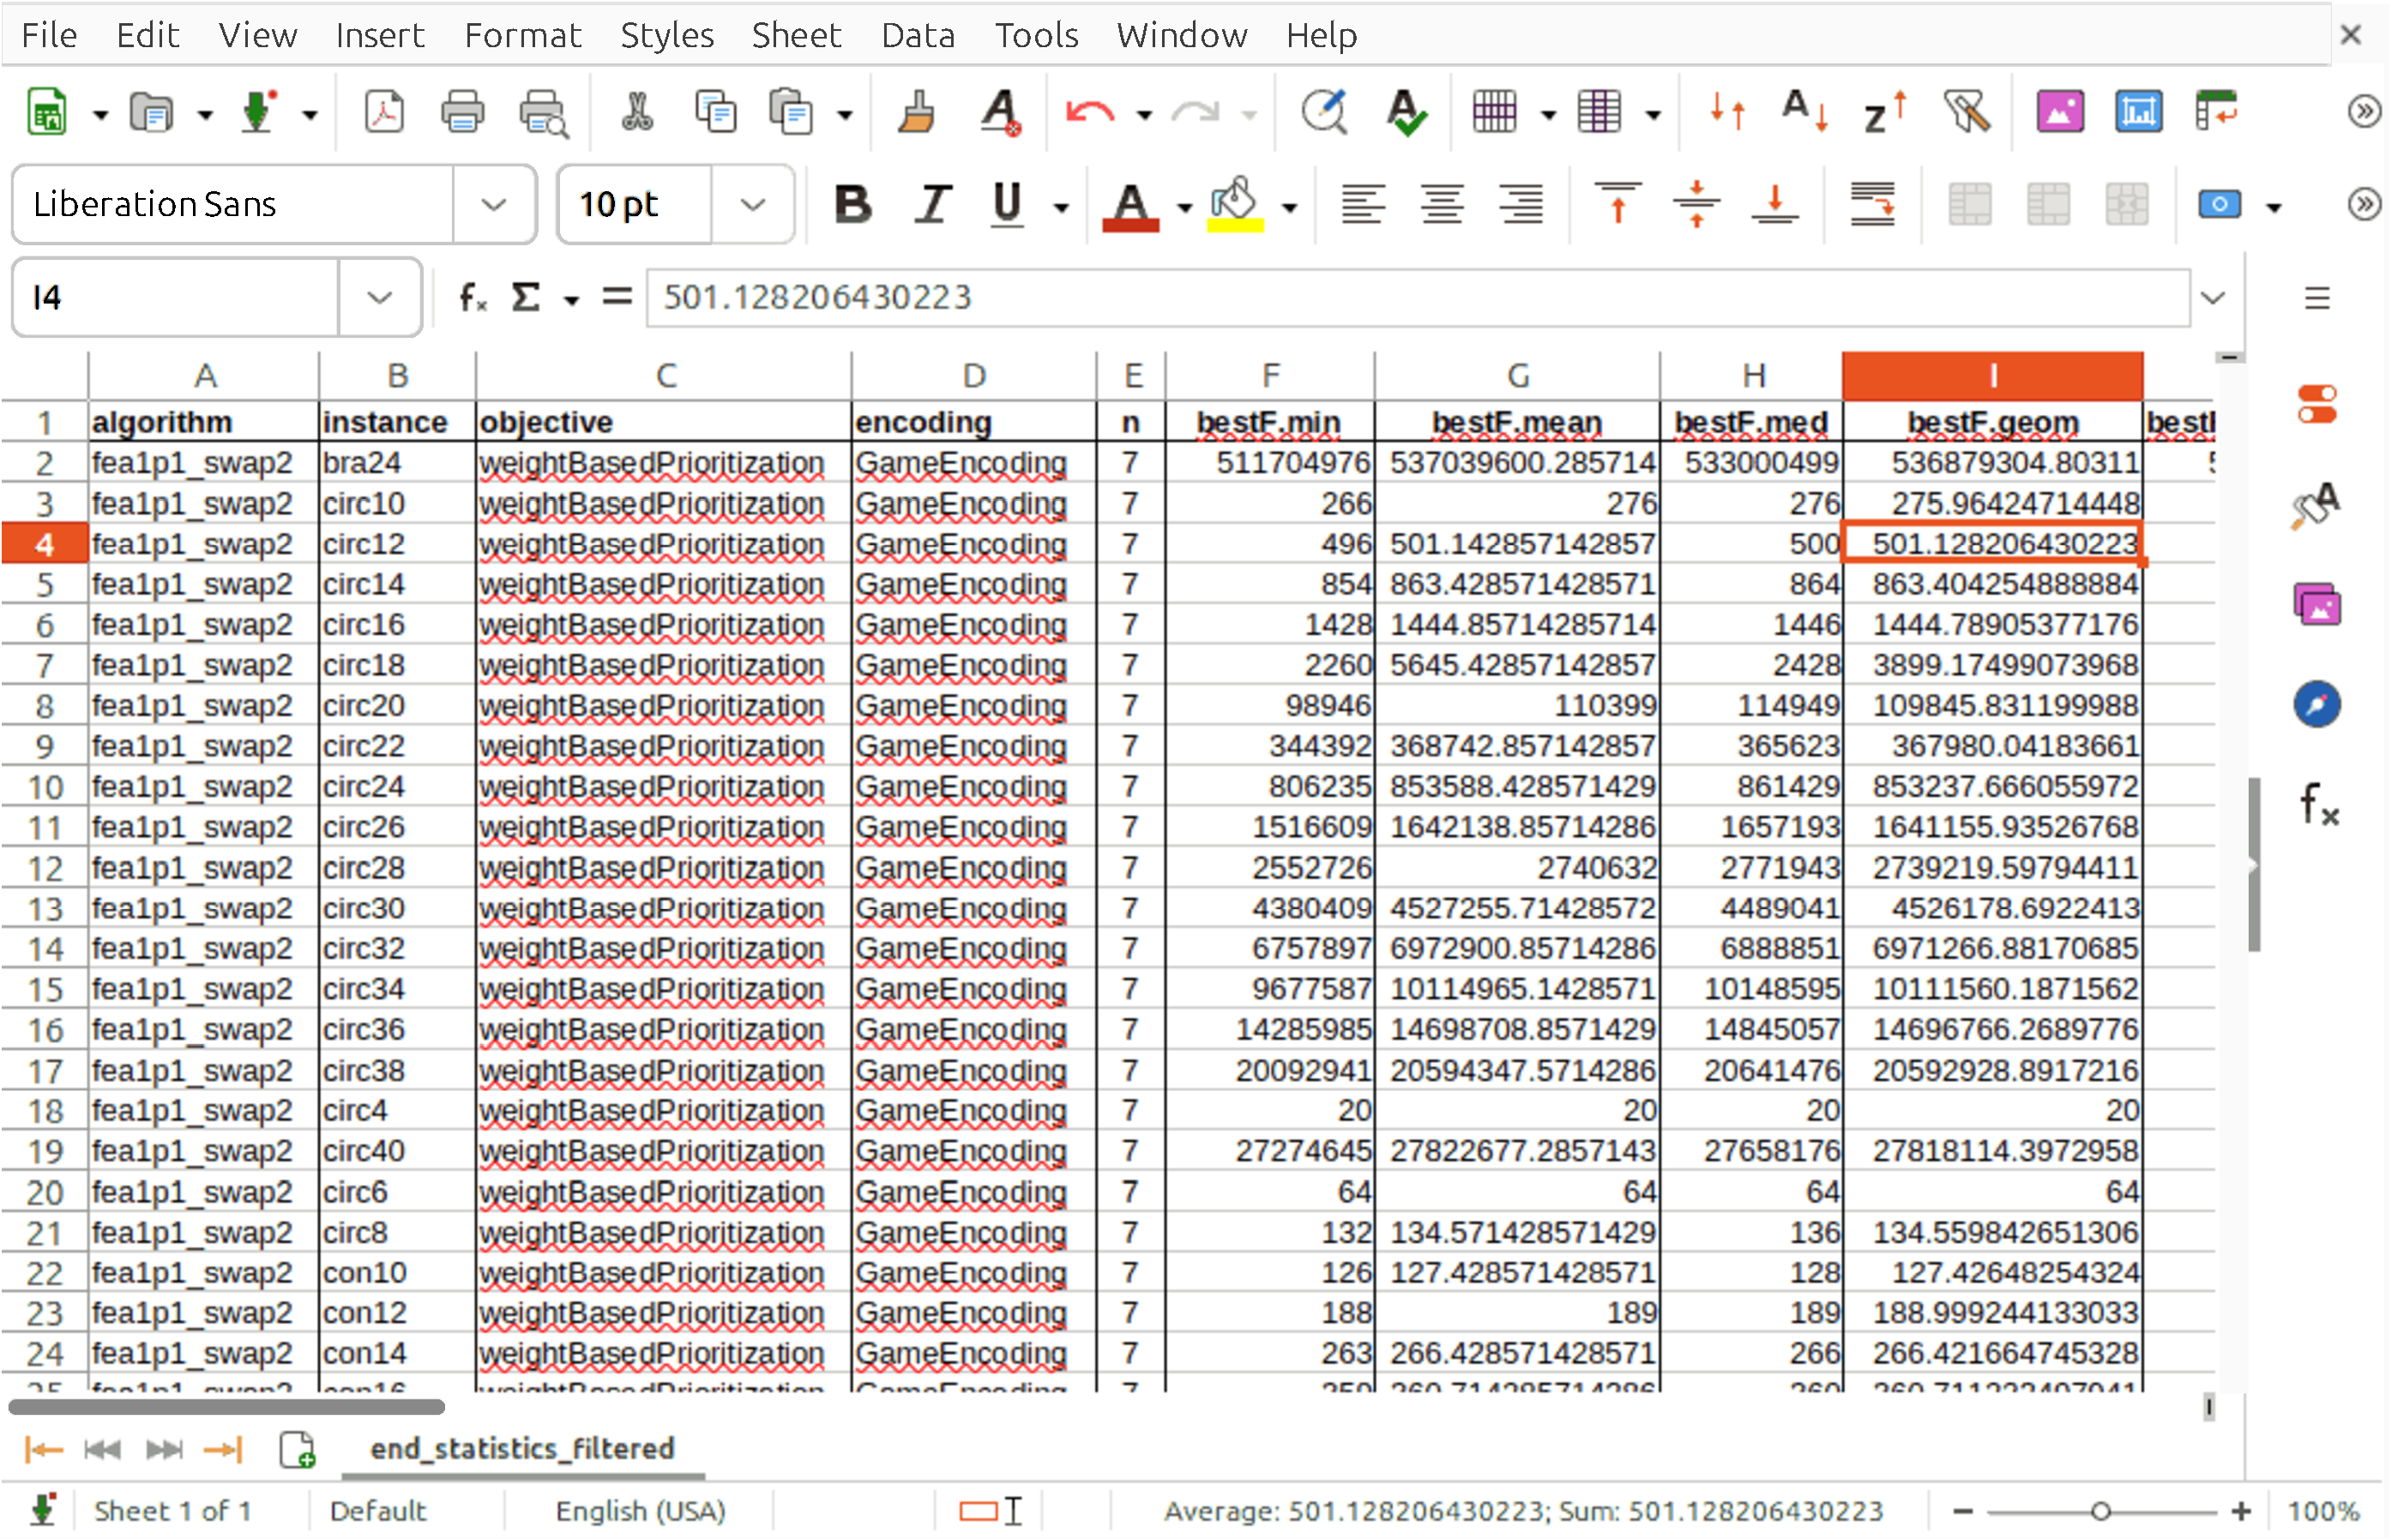
\includegraphics[width=0.6\linewidth]{\currentDir/libreOfficeCalc}}%
\caption{An example of tabular data, namely a \pgls{CSV} file opened and edited in \libreofficeCalc.}%
\label{fig:libreOfficeCalc}%
\end{figure}%
%
\begin{figure}%
\centering%
%
\subfloat[][%
An example of data stored in the \pgls{XML}.%
\label{fig:xmlexample}%
]{\tightbox{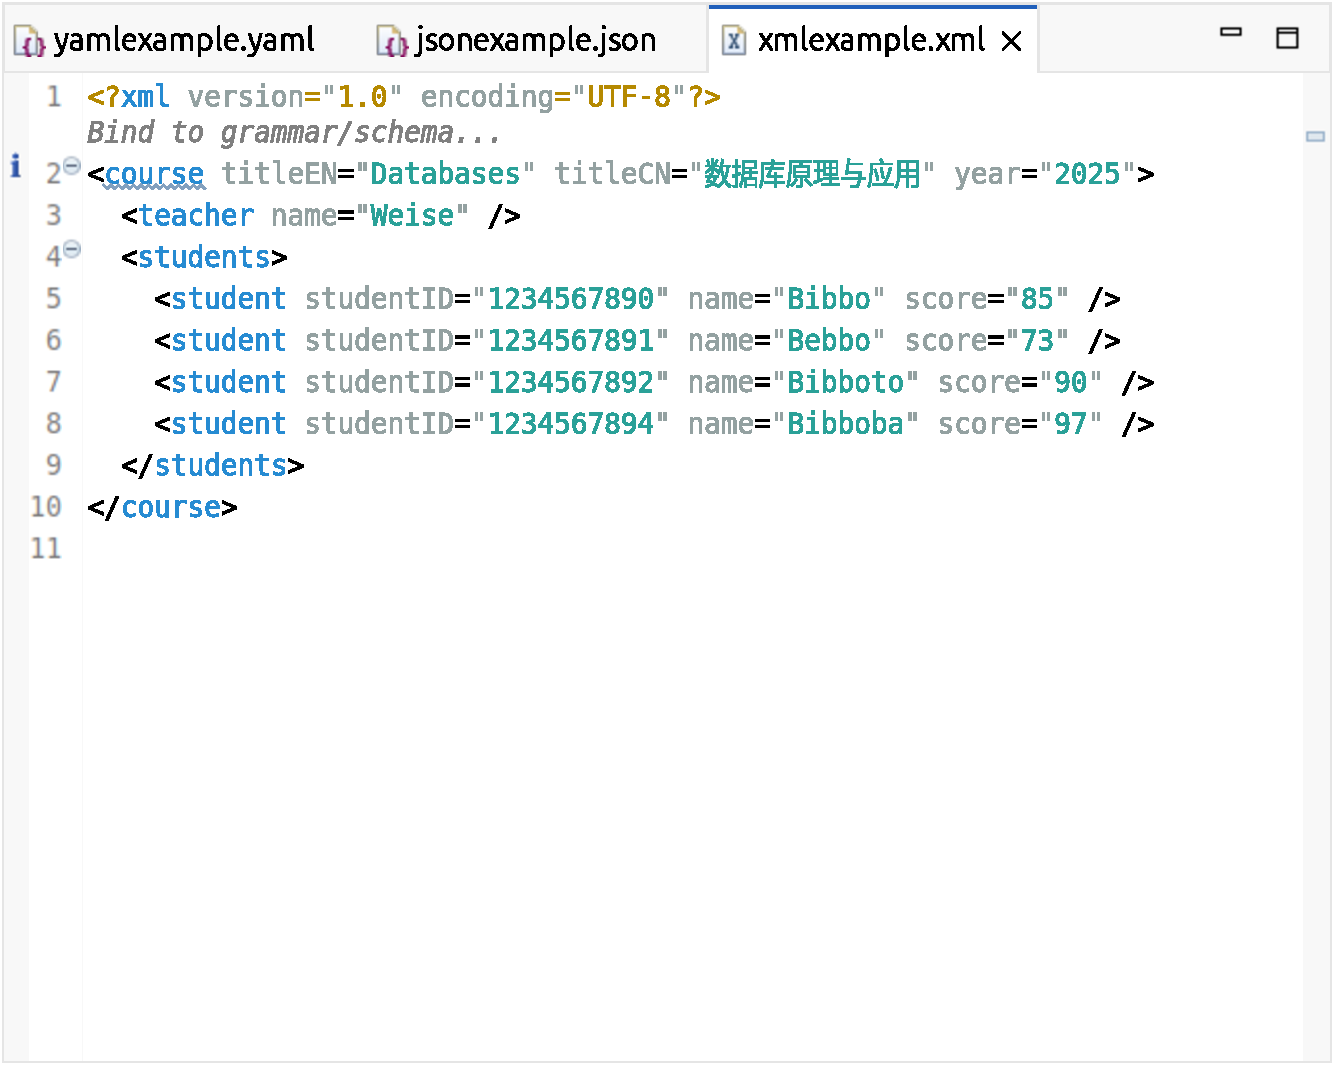
\includegraphics[width=0.325\linewidth]{\currentDir/xmlexample}}}%
%
\floatSep%
%
\subfloat[][%
An example of data stored in the \pgls{JSON}.%
\label{fig:jsonexample}%
]{\tightbox{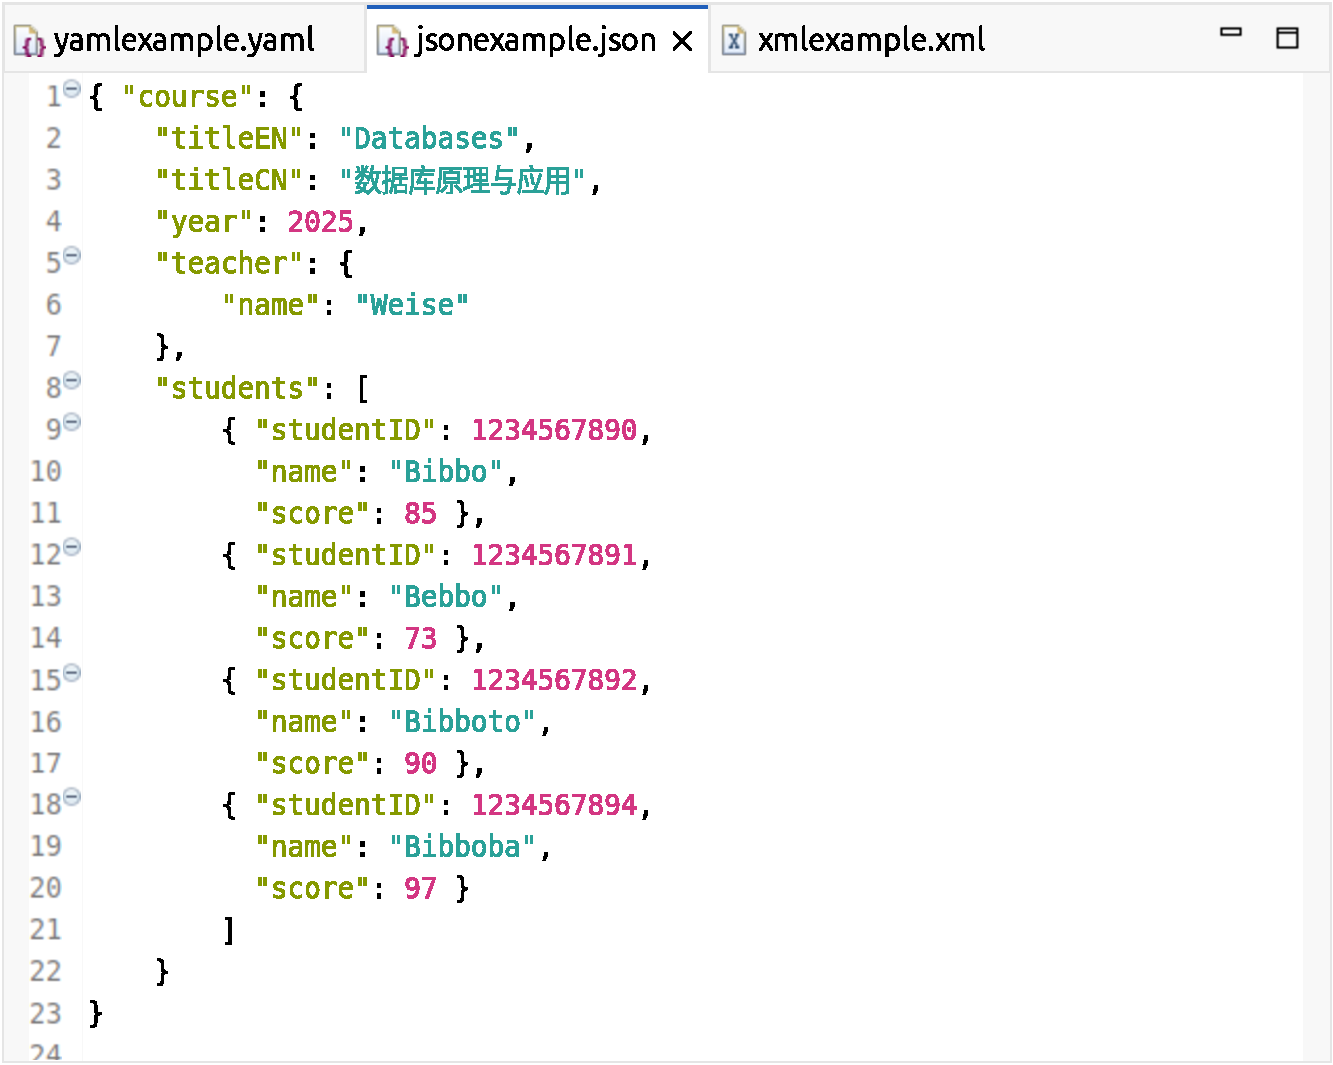
\includegraphics[width=0.325\linewidth]{\currentDir/jsonexample}}}%
%
\floatSep%
%
\subfloat[][%
An example of data stored in the \pgls{YAML}.%
\label{fig:yamlexample}%
]{\tightbox{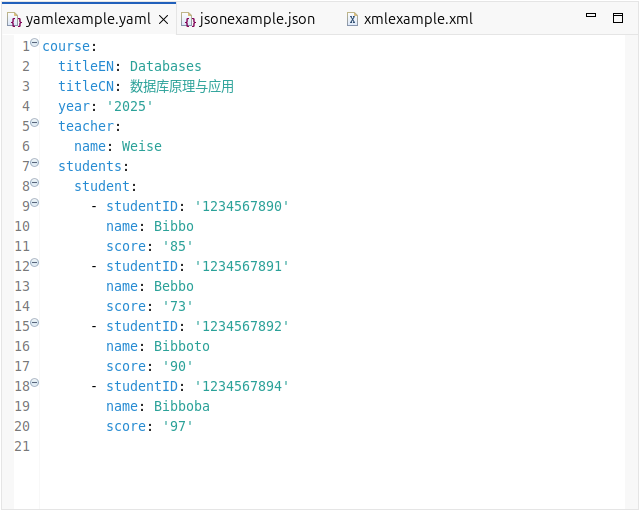
\includegraphics[width=0.325\linewidth]{\currentDir/yamlexample}}}%
%
\caption{Examples of the same dataset describing a course, its teachers, and the scores achieved by some of its student, presented in the dataformats \pgls{XML}, \pgls{JSON}, and \pgls{YAML}}.%
\label{fig:treeDataStructures}%
\end{figure}%
%
There are many different kinds of data.%
Since these kinds differ very much in their nature, the ways in which we store and retrieve them vary as well.

For example, there is unstructured data, like texts, graphics, or this book, as illustrated in~\cref{fig:documentDataProgrammingWithPython}.
Such unstructured pieces of data are usually stored in single document files.
An organization, e.g., a company or a university, produces heaps of such documents.
Every year, the students of our university write Bachelor's and Master's theses.
The different schools of our university submit reports, presentations, budget plans, and so on.
The university itself issues regulations and notices.
There exist common structures for the different document types in our university, such as templates for theses.
However, beyond such common structures, the data in the documents can vary enormously and there is no way to unify it.
Therefore, we \inQuotes{store} such data as singular documents and maybe organize these documents in catalogs, e.g., by student~ID, year, school, department, title, keyword, and so on.
If we want to retrieve the data from the theses, we can maybe search them by title or keyword.
Once we found the right document, we arrive at the end of what traditional technology can offer us and we have to read them.
Nowadays, maybe we can generate a summary using an \pgls{AI}, but in the end, we still have unstructured information to digest.

Then, there is data that is tightly structured and self-contained.
For data that can be stored in a single table, simple text formats like \gslreset{CSV}\pgls{CSV}~\cite{RFC4180} or \microsoftExcel~\cite{B2023DMWME,G2024ECRFMME} and \libreofficeCalc~\cite{S2022L7PFEUU,DF2024LTDF} tables are common.
One example is given in \cref{fig:libreOfficeCalc}.
If the data is more complex, maybe hierarchically structured, formats like \glsreset{XML}\pgls{XML}~\cite{BPSMM2008EMLX1FE,K2019ITXJY,CH2013XFCAMLTMC}, \glsreset{JSON}\pgls{JSON}~\cite{E2017SE4TJDIS,RFC8259}, or \glsreset{YAML}\pgls{YAML}~\cite{DNMAASBE2021YAMLYV1,K2019ITXJY,CGTYB2022YFFDCAIE} may be more suitable.
Examples of these formats are given in \cref{fig:treeDataStructures}.

All of these formats have in common that they store data in singular documents.
They offer clear and strict rules how the data can be defined, structured, stored, and retrieved.
They are open standards and vendor-independent.
With the exception of \microsoftExcel\ tables, they are also text-based formats.\footnote{%
Today, \microsoftExcel\ tables are stored as compressed collections of \pgls{XML} documents.%
} %
However, they are mainly suitable for data that, well, can be stored in single files efficiently.
They are not suitable for manipulating huge datasets.
They are also not suitable for modelling more complex relationships between different datasets.

For example, if we want to represent all the personnel, schools, students, and assets of our university, we could try to do that in a single \pgls{XML}~document.
This document would need to store which teacher belongs to which school, which student belongs to which school, which student is supervised by which teacher, and so on.
This \emph{can} be done.
Maybe a single person could write such a document.
But as soon as multiple people need to work on such a document together, everything will collapse.
Also, the document will be \emph{huge}.
Finding something or changing something will be incredibly tedious.
If an error occurs, maybe a misplaced character, maybe an unescaped quotation mark, then the whole document will no longer be valid.
Clearly, another way to work with \emph{relational} data is needed.
